\begin{intersong}
    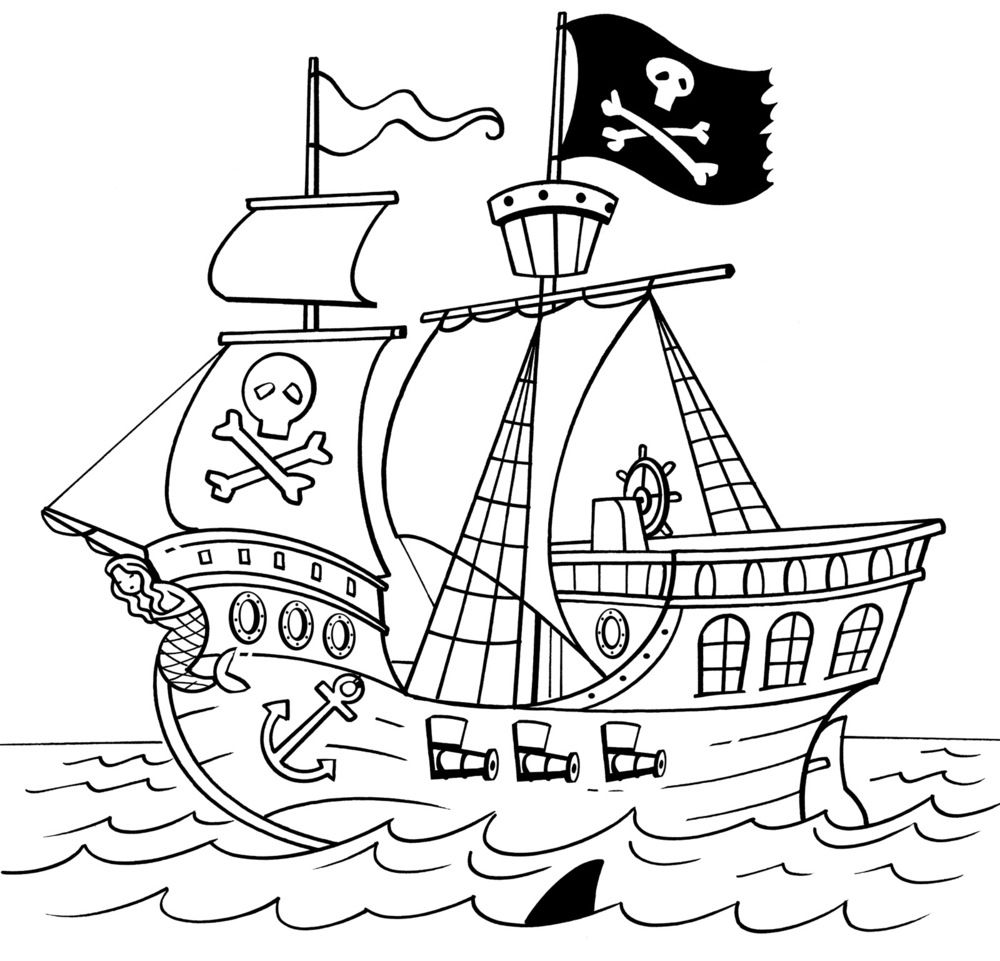
\includegraphics[width=0.4\textwidth]{triomfantelijkliedvandezilvervloot}
\end{intersong}
\beginsong{Triomfantelijk lied van de zilvervloot}
\beginverse*
Heb je van al gehoord van de Zilveren Vloot
De Zilveren Vloot van Spanje?
Die hadden veel Spaanse matten aan boord
En appeltjes van Oranje!
Piet Hein, Piet Hein,
Piet Hein zijn naam is klein,
Zijn daden bennen groot: (bis)
Die heeft gewonnen de Zilveren Vloot,
Die heeft gewonnen, gewonnen de Zilvervloot.
\endverse
\beginverse*
Zei toen niet Piet Hein met aalwarig woord:
"Wel jongetjes van Oranje,
Kom klim'reis aan dit en dat Spaanse boord
en rol met de matten van Spanje!"
Piet Hein, enz...
\endverse
\beginverse*
Klommen niet de jongens als katten in 't want
En vochten ze niet als leeuwen?
Ze maakten de Spanjers duchtig te schand
Tot Spanje klonk hun schreeuwen.
Piet Hein, enz…
\endverse
\beginverse*
Kwam er nu nog eenmaal zo'n Zilveren Vloot
Zeg, zou jullie nog zo kloppen?
Of zoudt gij u veilig buiten schoot
Maar stil in je hangmat stoppen?
"Wel Neerlands bloed,
Dat bloed heeft nog wel moed!
Al bennen we niet groot, (bis)
We zoùen winnen een Zilveren Vloot
We zoùen winnen, nog winnen een Zilvervloot!"
\endverse
\endsong